\documentclass[10pt]{article}
\usepackage[french]{babel}
\usepackage[utf8]{inputenc}
\usepackage[T1]{fontenc}
\usepackage{amsmath}
\usepackage{amsfonts}
\usepackage{amssymb}
\usepackage[version=4]{mhchem}
\usepackage{stmaryrd}
\usepackage{graphicx}
\usepackage[export]{adjustbox}
\graphicspath{ {./images/} }

\begin{document}
\section*{Analyse Numérique - correction TD n \({ }^{\boldsymbol{\circ}} \mathbf{3}\) 05-03-2025}
\section*{Exercice 1:}
Soit l'équation différentielle ordinaire utilisant une fonction \(y(t)\) :

\[
\frac{d y}{d t}=2 y-t-1 \quad \text { avec } \quad y(t=0)=1
\]

\begin{enumerate}
  \item Discrétiser l'équation en utilisant le schéma d'Euler Explicite (h est le pas de discrétisation)
\end{enumerate}

\[
\begin{aligned}
& y_{n+1}=y_{n}+h f\left(t_{n}, y_{n}\right) \\
& \frac{d y}{d t} \approx \frac{y_{n+1}-y_{n}}{h}=2 y_{n}-t_{n}-1
\end{aligned}
\]

D'où :

\[
y_{n+1}=y_{n}+h\left(2 y_{n}-t_{n}-1\right) \quad \text { et } \quad y_{0}=1
\]

\begin{enumerate}
  \setcounter{enumi}{1}
  \item Discrétiser l'équation en utilisant le schéma d'Euler Implicite\\
\(y_{n+1}=y_{n}+h f\left(t_{n+1}, y_{n+1}\right)\)\\
\(y_{n+1}=y_{n}+h\left(2 y_{n+1}-t_{n+1}-1\right)\)\\
Sachant que \(t_{n+1}=t_{n}+h\)\\
\(y_{n+1}(1-2 h)=y_{n}+h\left(-t_{n}-h-1\right)\)
\end{enumerate}

D'où :

\[
y_{n+1}=\frac{1}{1-2 h}\left(y_{n}+h\left(-t_{n}-h-1\right)\right) \quad \text { et } \quad y_{0}=1
\]

\begin{enumerate}
  \setcounter{enumi}{2}
  \item Discrétiser l'équation en utilisant le schéma de Runge-Kutta d'ordre 2\\
\(y_{n+1}=y_{n}+\frac{h}{2}\left(k_{1}+k_{2}\right)\)\\
Avec: \(\left\{\begin{array}{c}k_{1}=f\left(t_{n}, y_{n}\right) \\ k_{2}=f\left(t_{n}+h, y_{n}+h k_{1}\right)\end{array}\right.\)
\end{enumerate}

\[
y_{n+1}=y_{n}+\frac{h}{2}\left(k_{1}+k_{2}\right) \text { avec }:\left\{\begin{array}{c}
k_{1}=2 y_{n}-t_{n}-1 \\
k_{2}=2\left(y_{n}+h k_{1}\right)-\left(t_{n}+h\right)-1
\end{array} \quad \text { et } \quad y_{0}=1\right.
\]

\begin{enumerate}
  \setcounter{enumi}{3}
  \item Discrétiser l'équation en utilisant le schéma de Runge-Kutta d'ordre 4\\
\(y_{n+1}=y_{n}+\frac{h}{6}\left(k_{1}+2 k_{2}+2 k_{3}+k_{4}\right)\)\\
Avec : \(\left\{\begin{array}{c}k_{1}=f\left(t_{n}, y_{n}\right) \\ k_{2}=f\left(t_{n}+\frac{1}{2} h, y_{n}+\frac{1}{2} h k_{1}\right) \\ k_{3}=f\left(t_{n}+\frac{1}{2} h, y_{n}+\frac{1}{2} h k_{2}\right) \\ k_{4}=f\left(t_{n}+h, y_{n}+h k_{3}\right)\end{array}\right.\)
\end{enumerate}

\[
y_{n+1}=y_{n}+\frac{h}{6}\left(k_{1}+2 k_{2}+2 k_{3}+k_{4}\right) \quad \text { avec }:\left\{\begin{array}{c}
k_{1}=2 y_{n}-t_{n}-1 \\
k_{2}=2\left(y_{n}+\frac{1}{2} h k_{1}\right)-\left(t_{n}+\frac{1}{2} h\right)-1 \\
k_{3}=2\left(y_{n}+\frac{1}{2} h k_{2}\right)-\left(t_{n}+\frac{1}{2} h\right)-1 \\
k_{4}=2\left(y_{n}+h k_{3}\right)-\left(t_{n}+h\right)-1
\end{array} \quad \text { et } \quad y_{0}=1\right.
\]

\section*{Exercice 2:}
Soit I'EDO : \(\frac{d^{2} x}{d t^{2}}=\frac{k}{m}(l-x)-\frac{\mu}{m} \frac{d x}{d t}-g\)\\
Avec les conditions initiales suivantes : \(x(t=0)=l \quad ; \quad \frac{d x}{d t}(t=0)=0\)

\begin{enumerate}
  \item En posant \(y(t)=x^{\prime}(t)\), on va discrétiser le problème en utilisant le schéma d'Euler Explicite :
\end{enumerate}

\[
\begin{aligned}
& X_{n+1}=X_{n}+h f\left(t_{n}, X_{n}\right) \\
& \text { Avec : } X_{n}=\left[\begin{array}{l}
x_{n} \\
y_{n}
\end{array}\right], \text { et les conditions initiales } X_{0}=\left[\begin{array}{l}
x_{0}=l \\
y_{0}=0
\end{array}\right]
\end{aligned}
\]

Pour chacun des termes de \(X_{n}\), on applique le schéma d'Euler Explicite :\\
\(\left\{\begin{array}{c}x_{n+1}=x_{n}+h y_{n} \\ y_{n+1}=y_{n}+h\left(\frac{k}{m}\left(l-x_{n}\right)-\frac{\mu}{m} y_{n}-g\right)\end{array} \quad\right.\) avec \(\quad\left\{\begin{array}{l}x_{0}=l \\ y_{0}=0\end{array}\right.\)\\
Soit sous forme matricielle :\\
\(X_{n+1}=X_{n}+h f\left(t_{n}, X_{n}\right) \quad\) et \(\quad X_{0}=\left[\begin{array}{l}l \\ 0\end{array}\right]\)\\
Avec : \(f\left(t_{n}, X_{n}\right)=\left[\begin{array}{c}y_{n} \\ \frac{k}{m}\left(l-x_{n}\right)-\frac{\mu}{m} y_{n}-g\end{array}\right]\)\\
2. \(\mathrm{k}=50 ; \mathrm{m}=0.5 \mathrm{~m} ; \mathrm{I}=0.4 \mathrm{~m} ; \mu=1.5 ; \mathrm{g}=9.81 \mathrm{~m} / \mathrm{s}^{2}\)

Le pas de temps constant sera de \(h=0.01 s\).

On obtient :

\[
\begin{array}{lll}
t=0.00 \mathrm{~s} & x 0=0.40000 \mathrm{~m} & y 0=0.00000 \mathrm{~m} / \mathrm{s} \\
t=0.01 \mathrm{~s} & x 1=0.40000 \mathrm{~m} & y 1=-0.09810 \mathrm{~m} / \mathrm{s} \\
t=0.02 \mathrm{~s} & x 2=0.39902 \mathrm{~m} & y 2=-0.19326 \mathrm{~m} / \mathrm{s} \\
t=0.03 \mathrm{~s} & x 3=0.39709 \mathrm{~m} & y 3=-0.28458 \mathrm{~m} / \mathrm{s} \\
t=0.04 \mathrm{~s} & x 4=0.39424 \mathrm{~m} & y 4=-0.37123 \mathrm{~m} / \mathrm{s}
\end{array}
\]

\begin{enumerate}
  \setcounter{enumi}{2}
  \item Discrétiser le problème en utilisant le schéma de Runge-Kutta d'ordre 2 (prédicteur-correcteur) :
\end{enumerate}

\[
X_{n+1}=X_{n}+\frac{h}{2}\left(K_{1}+K_{2}\right) \quad \text { avec }\left\{\begin{array}{c}
K_{1}=f\left(t_{n}, X_{n}\right) \\
K_{2}=f\left(t_{n}+h, X_{n}+h K_{1}\right)
\end{array}\right.
\]

II faut écrire les vecteurs \(K_{1}\) et \(K_{2}:\)

\[
\begin{aligned}
& K_{1}=f\left(t_{n}, X_{n}\right)=\left[\begin{array}{l}
k_{1 x} \\
k_{1 y}
\end{array}\right] \quad \text { avec : }\left\{\begin{array}{c}
k_{1 x}=y_{n} \\
k_{1 y}=\frac{k}{m}\left(l-x_{n}\right)-\frac{\mu}{m} y_{n}-g
\end{array}\right. \\
& K_{2}=f\left(t_{n}+h, X_{n}+h K_{1}\right)=\left[\begin{array}{l}
k_{2 x} \\
k_{2 y}
\end{array}\right] \quad \text { avec } X_{n}+h K_{1}=\left[\begin{array}{l}
x_{n} \\
y_{n}
\end{array}\right]+h\left[\begin{array}{l}
k_{1 x} \\
k_{1 y}
\end{array}\right]=\left[\begin{array}{l}
x_{n}+h k_{1 x} \\
y_{n}+h k_{1 y}
\end{array}\right]
\end{aligned}
\]

On obtient alors :

\[
\left\{\begin{array}{c}
k_{2 x}=y_{n}+h k_{1 y} \\
k_{2 y}=\frac{k}{m}\left(l-\left(x_{n}+h k_{1 x}\right)\right)-\frac{\mu}{m}\left(y_{n}+h k_{1 y}\right)-g
\end{array}\right.
\]

\section*{Exercice 3:}
\begin{enumerate}
  \item Rappel du développement de Taylor :
\end{enumerate}

\[
f(x+\Delta x)=f(x)+\sum_{k=1}^{n} \frac{f^{(k)}(x)}{k!}(\Delta x)^{k}+\Theta\left(\Delta x^{n+1}\right)
\]

Ecrivons les développements :\\
(2) \(f(x-h)=f(x)-h \frac{d f}{d x}+\frac{h^{2}}{2} \frac{d^{2} f}{d x^{2}}-\frac{h^{3}}{6} \frac{d^{3} f}{d x^{3}}+\theta\left(h^{4}\right)\)\\
(3) \(f(x+h)=f(x)+h \frac{d f}{d x}+\frac{h^{2}}{2} \frac{d^{2} f}{d x^{2}}+\frac{h^{3}}{6} \frac{d^{3} f}{d x^{3}}+\theta\left(h^{4}\right)\)\\
(4) \(f(x+2 h)=f(x)+2 h \frac{d f}{d x}+\frac{4 h^{2}}{2} \frac{d^{2} f}{d x^{2}}+\frac{8 h^{3}}{6} \frac{d^{3} f}{d x^{3}}+\theta\left(h^{4}\right)\)

Etablissement du schéma pour la dérivée seconde sur 3 points :\\
Additionnons les équations (2) et (3) :

\[
\begin{aligned}
& f(x-h)+f(x+h)=2 f(x)+h^{2} \frac{d^{2} f}{d x^{2}}+\theta\left(h^{4}\right) \\
& \quad \rightarrow \frac{d^{2} f}{d x^{2}}=\frac{1}{h^{2}}(f(x-h)+f(x+h)-2 f(x))+\theta\left(h^{2}\right) \\
& \rightarrow D_{x x}^{0}=\frac{1}{h^{2}}\left(f_{i-1}-2 f_{i}+f_{i+1}\right)
\end{aligned}
\]

Etablissement du schéma pour la dérivée seconde sur 5 points : Additionnons les 4 équations :

\[
\begin{aligned}
& f(x-2 h)+f(x-h)+f(x+h)+f(x+2 h)=4 f(x)+10 \frac{h^{2}}{2} \frac{d^{2} f}{d x^{2}}+\theta\left(h^{4}\right) \\
& \rightarrow \frac{d^{2} f}{d x^{2}}=\frac{1}{h^{2}}(f(x-2 h)+f(x-h)-4 f(x)+f(x+h)+f(x+2 h))+\theta\left(h^{2}\right) \\
& \rightarrow \widetilde{D}_{x x}^{0}=\frac{1}{5 h^{2}}\left(f_{i-2}+f_{i-1}-4 f_{i}+f_{i+1}+f_{i+2}\right)
\end{aligned}
\]

\section*{Vérification de la validité des schémas obtenus:}
Déterminons par exemple la dérivée seconde pour la fonction \(f(x)=a x^{2}+b\)\\
\(\frac{d f}{d x}=2 a x\) et \(\frac{d^{2} f}{d x^{2}}=2 a\)\\
\(\widetilde{D}_{x x}^{0}=\frac{1}{h^{2}}\left(a(x-h)^{2}+b-2\left(a x^{2}+b\right)+a(x+h)^{2}+b\right)\)\\
Après développement on, obtient bien \(D_{x x}^{0}=2 a\)\\
Même constat avec le schéma à 5 points : \(\widetilde{D}_{x x}^{0}=2 a\)\\
Ce qui valide nos schémas de dérivée seconde \(\widetilde{D}_{x x}^{0}\) et \(D_{x x}^{0}\)\\
2. On a :

\[
T=2100 \mathrm{~N}, q=12600 \mathrm{~N} / \mathrm{m}, L=12 \mathrm{~m}, \mathrm{E}=210 \mathrm{e} 9 \mathrm{~Pa} \text { et } I_{z}=0.0001 \mathrm{~m}^{4}
\]

En remplaçant les coefficients de l'EDP par leurs valeurs numériques, on a:

\[
\begin{aligned}
& \frac{d^{2} y}{d x^{2}}-\frac{2100 y}{210 e 5}=\frac{(12600) x(12-x)}{420 e 5} \\
& \quad \frac{d^{2} y}{d x^{2}}-(1 \mathrm{e}-04) y=(3 e-4) x(12-x)
\end{aligned}
\]

La dérivée seconde \(\frac{d^{2} y}{d x^{2}}\) au nœud \(i\) est approchée par une différence divisée centrée,\\
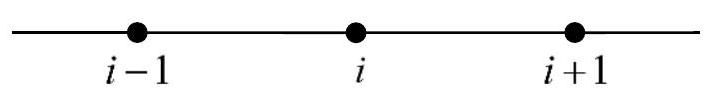
\includegraphics[max width=\textwidth, alt={}, center]{61b61817-c95f-48db-8eb4-9f2412ea02e8-4_101_714_1576_641}

\[
\frac{d^{2} y}{d x^{2}} \approx \frac{y_{i+1}-2 y_{i}+y_{i-1}}{\Delta x^{2}}
\]

L'équation est réécrite de la façon suivante :

\[
\frac{y_{i+1}-2 y_{i}+y_{i-1}}{\Delta x^{2}}-(1 e-04) y_{i}=(3 e-04) x_{i}\left(12-x_{i}\right)
\]

\begin{enumerate}
  \setcounter{enumi}{2}
  \item On choisit les conditions limites de Dirichlet suivantes
\end{enumerate}

\begin{itemize}
  \item \(y(x=0)=0\), on a alors \(y_{1}=0\)
  \item \(y(x=12)=0\) on a alors \(y_{N}=0\)
\end{itemize}

Calcul du pas spatial \(\Delta x\) :\\
On a \(\Delta x=\frac{L}{N-1}=\frac{12}{7-1}=2 \mathrm{~m}\)\\
Calcul des différents noeuds

\[
x_{1}=0
\]

\[
\begin{aligned}
& x_{2}=x_{1}+\Delta x=0+2=2 \mathrm{~m} \\
& x_{3}=x_{2}+\Delta x=2+2=4 \mathrm{~m} \\
& x_{4}=x_{3}+\Delta x=4+2=6 \mathrm{~m} \\
& x_{5}=x_{4}+\Delta x=6+2=8 \mathrm{~m} \\
& x_{6}=x_{5}+\Delta x=8+2=10 \mathrm{~m} \\
& x_{7}=x_{6}+\Delta x=10+2=12 \mathrm{~m}
\end{aligned}
\]

Noeud 1 : à partir de la condition limite pour \(x_{1}=0\), on obtient :

\[
y_{1}=0
\]

Noeud 2 : pour le noeud 2, on a :

\[
\frac{y_{3}-2 y_{2}+y_{1}}{(2)^{2}}-(1 . e-04) y_{2}=(3 . e-4) x_{2}\left(12-x_{2}\right)
\]

\[
0.25 y_{3}-0.5001 y_{2}+0.25 y_{1}=(36 . e-04) x_{2}-(3 e-04) x_{2}^{2}
\]

Noeud 3 : pour le noeud 3 , on obtient l'équation suivante :

\[
\begin{array}{r}
\frac{y_{4}-2 y_{3}+y_{2}}{(2)^{2}}-(1 . \mathrm{e}-04) y_{3}=(3 e-4) x_{3}\left(12-x_{3}\right) \\
0.25 y_{4}-0.5001 y_{3}+0.25 y_{2}=(36 . \mathrm{e}-04) x_{3}-(3 \mathrm{e}-04) x_{3}^{2}
\end{array}
\]

Noeuds 4 5,6 : Même équations avec indices évolutifs

Nœud 7 : A partir de la condition limite à \(x=12\), on obtient :

\[
y_{7}=0
\]

\begin{enumerate}
  \setcounter{enumi}{3}
  \item A partir des 7 équations précédentes, on obtient le système matriciel suivant de type \(\mathrm{A} \mathrm{x}=\mathrm{b}\)
\end{enumerate}

\[
\left[\begin{array}{ccccccc}
1 & 0 & 0 & 0 & 0 & 0 & 0 \\
0.25 & -0.5001 & 0.25 & 0 & 0 & 0 & 0 \\
0 & 0.25 & -0.5001 & 0.25 & 0 & 0 & 0 \\
0 & 0 & 0.25 & -0.5001 & 0.25 & 0 & 0 \\
0 & 0 & 0 & 0.25 & -0.5001 & 0.25 & 0 \\
0 & 0 & 0 & 0 & 0.25 & -0.5001 & 0.25 \\
0 & 0 & 0 & 0 & 0 & 0 & 1
\end{array}\right]\left[\begin{array}{l}
y_{1} \\
y_{2} \\
y_{3} \\
y_{4} \\
y_{5} \\
y_{6} \\
y_{7}
\end{array}\right]=\left[\begin{array}{c}
0 \\
0.006 \\
0.0096 \\
0.0108 \\
0.0096 \\
0.006 \\
0
\end{array}\right]
\]

On utilise par exemple une méthode itérative pour résoudre le système matriciel. On a alors la solution suivante :

\[
\left[\begin{array}{l}
y_{1} \\
y_{2} \\
y_{3} \\
y_{4} \\
y_{5} \\
y_{6} \\
y_{7}
\end{array}\right]=\left[\begin{array}{c}
0 \\
-0.083876 \\
-0.143785 \\
-0.165352 \\
-0.143785 \\
-0.083876 \\
0
\end{array}\right]
\]

\begin{enumerate}
  \setcounter{enumi}{4}
  \item On a \(y(8)=y\left(x_{5}\right) \approx y_{5}=-0,143785 m\) soit environ -144 mm
  \item La solution exacte est donnée par :
\end{enumerate}

\[
y(x)=C_{1} \exp (x / 100)+C_{2} \exp (-x / 100)+3 x^{2}-36 x+60000
\]

A partir des conditions limites choisies, on obtient :

\[
y(x)=-28202.1569 \exp (x / 100)-31797.8431 \exp (-x / 100)+3 x^{2}-36 x+60000
\]

On a alors

\[
y(8)=-0.140596 \mathrm{~m}
\]

L'erreur totale est :

\[
\begin{aligned}
& E_{t}=\text { Valeur exacte }- \text { Valeur approchée } \\
& E_{t}=-0.140595-(-0.143785) \\
& E_{t}=3.19 \times 10^{-3} \mathrm{~m}
\end{aligned}
\]

L'erreur relative est égale à :

\[
\begin{aligned}
& E=\frac{\left|y_{\text {exacte }}-y\right|}{\left|y_{\text {exacte }}\right|} \times 100 \\
& E=\frac{3.19 \times 10^{-3}}{0.140596} \times 100 \\
& E=2.27 \%
\end{aligned}
\]


\end{document}